\chapter{Una hora escrita con Sol -- II}

\vfill

\lettrine[lines=2]{A}{l día siguiente}, Antonia esperaba a Cecilia con
im\-pa\-cie\-ncia: ---¡Por fin llegaste! ---saludó, fingiendo burlona
intranquilidad.

---No te preocupes ---respondió su amiga con una son\-ri\-sa---; en
cuanto imprimamos nuestro reloj podrás medir con precisión mi
impuntualidad... al menos cuando no esté nublado.

Cecilia se sentó frente a la computadora con menos entusiasmo que de
costrumbre; quizás ella también, ante la inminente finalización de
esta aventura, estaba sintiendo una nostalgia anticipada.

Antonia, según su costumbre, pareció no notarlo:

---Ya sabemos cómo calcular el ángulo con el que debemos escorzar
nuestros dígitos a cada hora puntual; sabemos también cómo rescatarlos
individualmente. Ahora parecería que sólo debemos ponerlos uno al lado
del otro, y recorrer las horas y minutos desde las 6:00 a las 18:00.

Antonia puso un énfasis involuntario en el último potencial, que
provocó en Cecilia una instintiva actitud defensiva: anticipó que otro
problema estaba por hacer su aparición.

\section{El separador}

\guillemotright En primer lugar, tenemos entonces que colocar los
cuatro dígitos que componen la hora uno al lado del otro ---continuó
Antonia.

---¡No te olvides del separador de horas y minutos!  ---in\-terrumpió
Cecilia que estaba alerta---. Las \texttt{1345} no parecen una hora
muy seria...

---Tenés razón ---admitió Antonia, sonriendo---.  Tenemos que hacerle
lugar también. No sólo en el reloj, sino en el texto: se merece su
propio módulo ---e inmediatamente deslizó sus dedos sobre el teclado.

\begin{lstlisting}
module separador(alfa){
  for(i=[-1,1])
    translate([i*0.5*(alto_pixel+delta_alto), 0, -.01])
      rayo_de_sol(alfa);
}  
difference(){
  rotate([-90,0,0])
    semicilindro(150,30,center=true);  
  separador(60);
  translate([0,-30,0])
    digito(60,2);
}
\end{lstlisting}%
\begin{figure}[ht]
  \centering
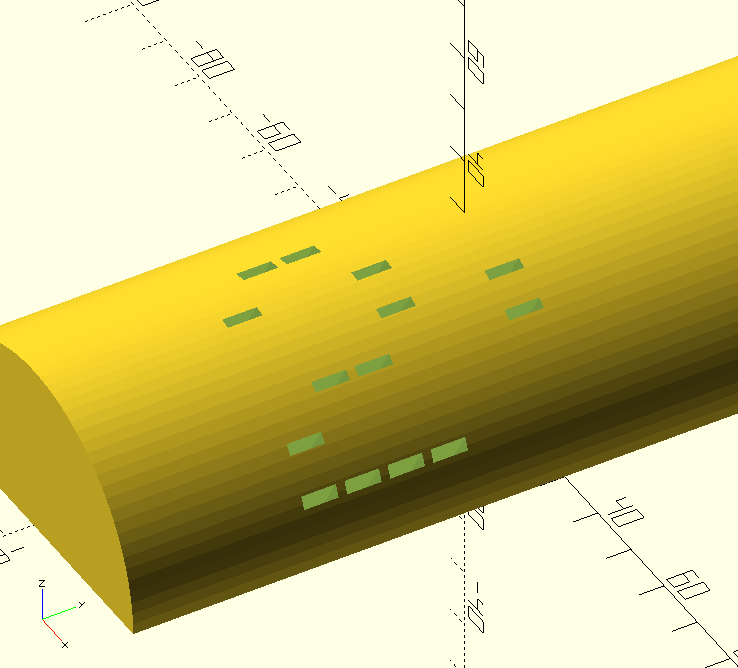
\includegraphics[width=.52\textwidth]{imagenes/separador}  
\caption[Separador I]{Primera versión del separador de horas y
  minutos.}
  \label{fig:separador}
\end{figure}


---¿Creo que no tiene mucho misterio, no? ---preguntó An\-to\-nia
re\-tó\-ri\-ca\-men\-te---. El separador consiste en dos rayos de Sol,
dispuestos vertical y simétricamente.

---Es cierto ---admitió Cecilia---; pero recordemos que nuestro
separador convivirá con la \lstinline!hora_solar!, que recibirá como
parámetros la hora y los minutos, no el ángulo ---agregó, mientras se
disponía a corregir el módulo de Antonia.

\begin{lstlisting}
module separador(horas,minutos){
  alfa=alfa(horas+minutos/60);
  for(i=[-1,1])
    translate([i*0.5*(alto_pixel+delta_alto), 0, -.01])
      rayo_de_sol(alfa);
}  
difference(){
  rotate([-90,0,0])
    semicilindro(150,30,center=true);  
  separador(14,0);
  translate([0,-30,0])
    digito(60,2);
}
\end{lstlisting}%
% \begin{figure}[ht]
%   \centering
% 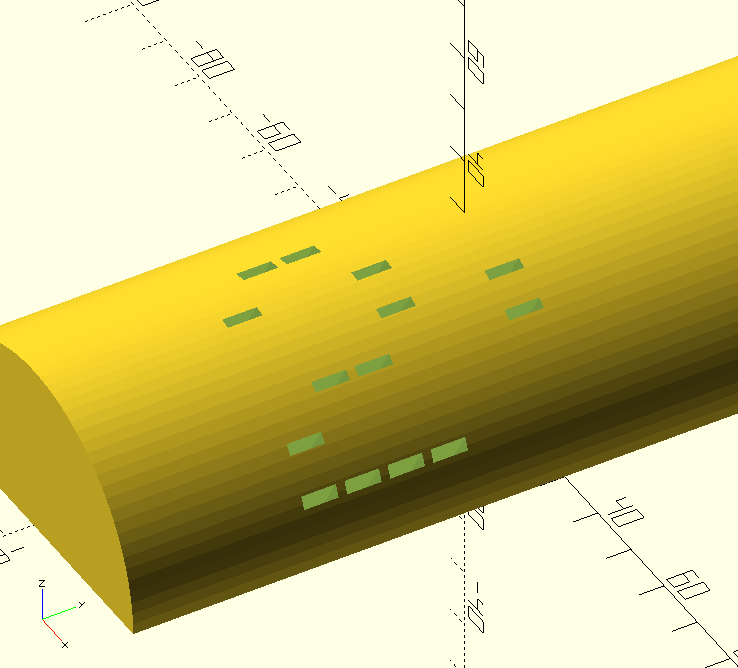
\includegraphics[width=.45\textwidth]{imagenes/separador}  
% \caption[Separador II]{Otra versión del separador de horas y
%   minutos.}
%   \label{fig:separador-2}
% \end{figure}


\guillemotright A las 14:00 les corresponden un ángulo de 60$^{\circ}$
en nuestro hemisferio; por eso el separador quedó alineado con el `2'
---co\-men\-tó Cecilia, mientras Antonia la miraba en silencio y como si
no la reconociese.

\section{El cuerpo del reloj}

Cecilia seguía mirando el texto con gesto de in\-sa\-tis\-fac\-ción:

---¿No te parece que el cuerpo del reloj ya está mereciendo también su
propio módulo?  Las crudas líneas 8 y 9 me parecen indignas de
convivir con el \lstinline!separador! y el \lstinline!digito!...  ---y
tras unos instantes, compartió con Antonia su nuevo módulo.

 %   \begin{center}
    \begin{lstlisting}
module cuerpo(largo){
  rotate([-90,0,0])
    semicilindro(largo,radio_semicilindro, center=true);  
}
difference(){
  cuerpo(150);
  separador(14,0);
  translate([0,-30,0])
    digito(60,2);
}
    \end{lstlisting}%
% \end{minipage}\hfill

%   \begin{minipage}[b]{.35\textwidth}\vspace{0pt}
    \begin{figure}[ht]
      \centering
       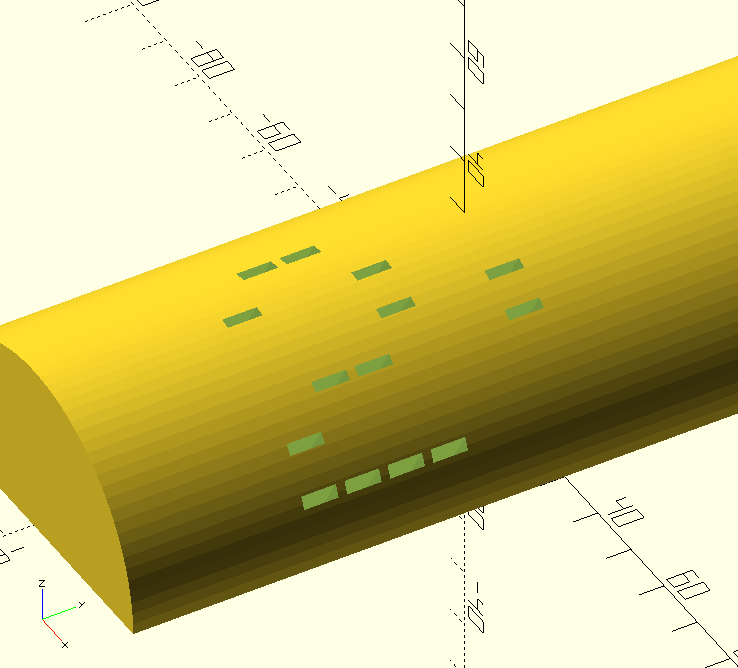
\includegraphics[width=.44\textwidth]{imagenes/separador}
       \caption{Cecilia otorga al cuerpo del reloj su merecido módulo
         propio.}
  \label{fig:separador-3}
\end{figure}
       % \end{minipage}
 %        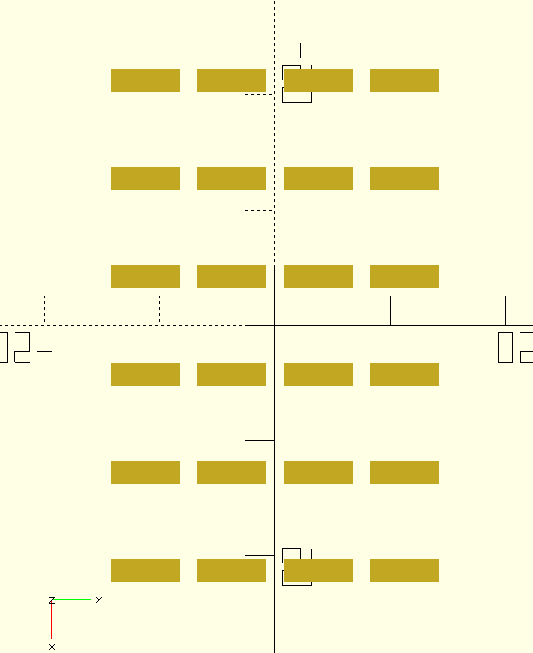
\includegraphics[width=3cm]{matriz-completa-centrada-0}


\section{La posición de los dígitos}

\subsection{Las horas}

Antonia recuperó el teclado casi con sigilo:

---Muy bien, Cecilia ---deslizó con suavidad---. Ahora sí, creo que
podemos tratar de colocar los dígitos; comencemos por la hora
---añadió, mientras elaboraba el sencillo boceto de la figura
\ref{fig:horas-completas-posiciones}.

\begin{figure}[ht]
  \centering
  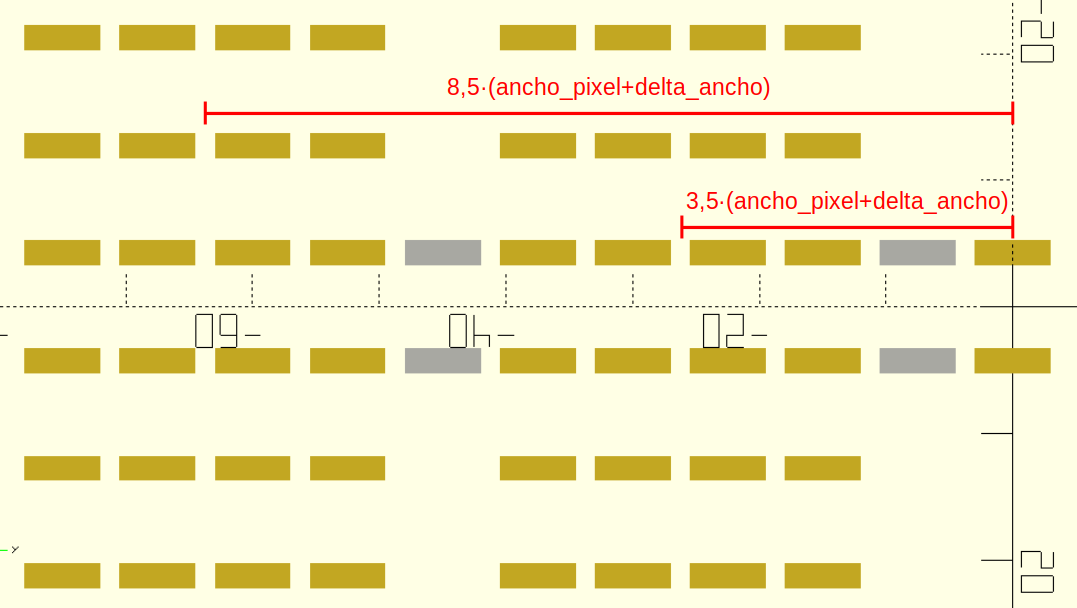
\includegraphics[width=1\textwidth]{imagenes/horas-completas-posiciones}
  \caption{Antonia calcula la posición de los dígitos de las horas.}
  \label{fig:horas-completas-posiciones}
\end{figure}



\guillemotright Agregué dos separadores `fantasmas' para ayudarnos a
calcular la ubicación de los centros de ambos dígitos; si no me
equivoco, las decenas de las horas se ubican a
\lstinline!8.5*(ancho_pixel + delta_ancho)! del origen de coordenadas,
mientras que las unidades están a \lstinline!3.5*(ancho_pixel + delta_ancho)! del mismo punto.

Cecilia recorrió con la punta de un dedo el monitor mientras contaba
en silencio: enseguida pudo confirmar los resultados de Antonia.

---Si te parece bien, no demoremos más en agregar las horas a nuestro
reloj... ---con una amplia sonrisa, Antonia sumó al módulo
\lstinline!hora_solar! la nueva conquista:


\begin{lstlisting}
module hora_solar(horas,minutos){
  alfa=alfa(horas+minutos/60);
  hora_decenas=n_a_digito(horas,1);
  hora_unidades=n_a_digito(horas,0);
  minuto_decenas=n_a_digito(minutos,1);
  minuto_unidades=n_a_digito(minutos,0);
                    
  delta_y=ancho_pixel+delta_ancho;
  translate([0,-8.5*delta_y,0])
    digito(alfa,hora_decenas);
  translate([0,-3.5*delta_y,0])
    digito(alfa,hora_unidades);  
}
difference(){
  cuerpo(170);
  separador(12,0);
  hora_solar(12,0);
}
\end{lstlisting}%

\begin{figure}[ht]
  \centering 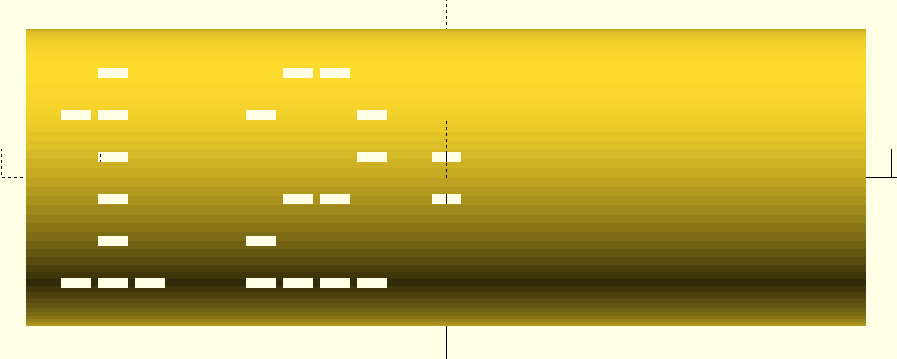
\includegraphics[width=.8\textwidth]{imagenes/12_00}
  \caption{Antonia agrega las horas al módulo \lstinline!hora_solar!.}
  \label{fig:12_00}
\end{figure}


Cecilia tuvo que reprimir un grito de alegría ante la figura
\ref{fig:12_00}: aún no se acostumbraba a que la realidad ---aun
tratándose de una realidad ``computacional''--- se adecuara fielmente
a las ideas y cálculos que elucubraban con Antonia. Se preguntó, no
sin inquietud, que sentiría cuando vieran al fin el reloj impreso,
como un objeto real y plenamente físico... Tomando para sí el teclado,
decidió probar el módulo con otras horas: las 9:00 y las 15:00.

\begin{lstlisting}
difference(){
  cuerpo(170);
  separador(9,0);
  hora_solar(9,0);
}
\end{lstlisting}%

\begin{figure}[ht]
    \centering
    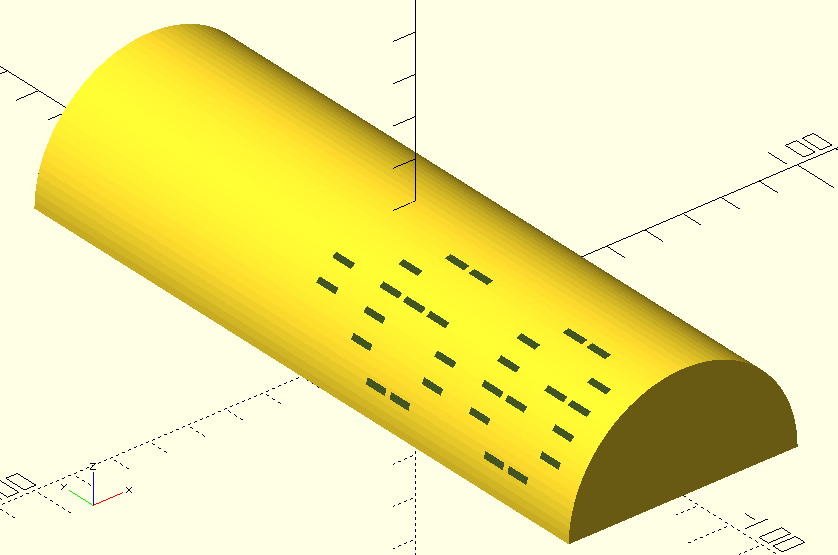
\includegraphics[width=.5\textwidth]{imagenes/9_00}
  \caption{Cecilia comprueba el módulo \lstinline!hora_solar! para las 9:00.}
\label{fig:9_00}
\end{figure}



\begin{lstlisting}
difference(){
  cuerpo(170);
  separador(15,0);
  hora_solar(15,0);
}
\end{lstlisting}%

\begin{figure}[ht]
    \centering
    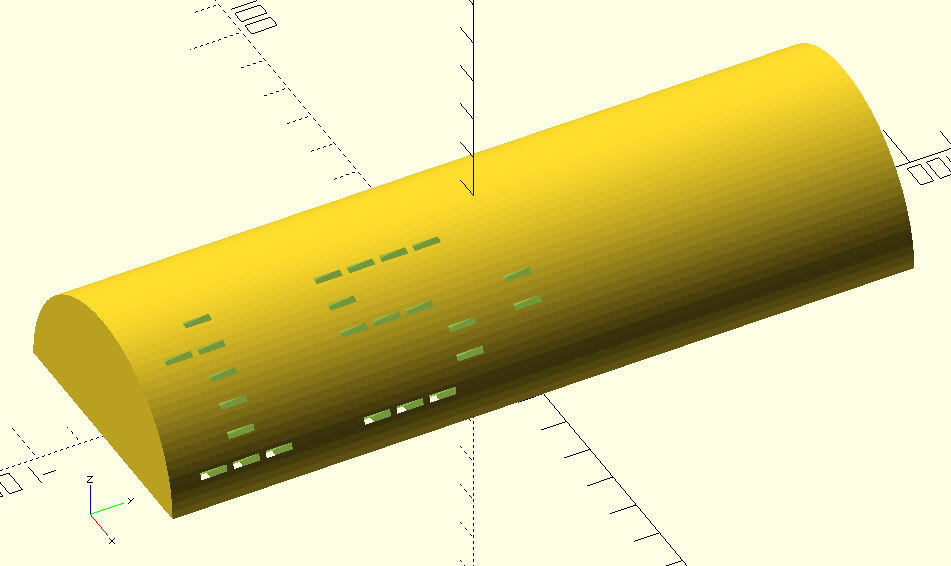
\includegraphics[width=.56\textwidth]{imagenes/15_00}
  \caption{Cecilia comprueba el módulo \lstinline!hora_solar! para las 15:00.}
\label{fig:15_00}
\end{figure}


Las 9:00 y las 15:00 inquietaron un poco a Cecilia: ¿No estaban
demasiado cerca de la base del reloj? Temió que más cerca de las 18:00
o de las 6:00 los dígitos se ``cayeran'' del mismo... Luego de unos
instantes de aprensión, se armó de coraje y decidió probar una hora
extrema:


\begin{lstlisting}
difference(){
  cuerpo(170);
  separador(17,0);
  hora_solar(17,0);
}
\end{lstlisting}%

\begin{figure}[ht]
  \centering 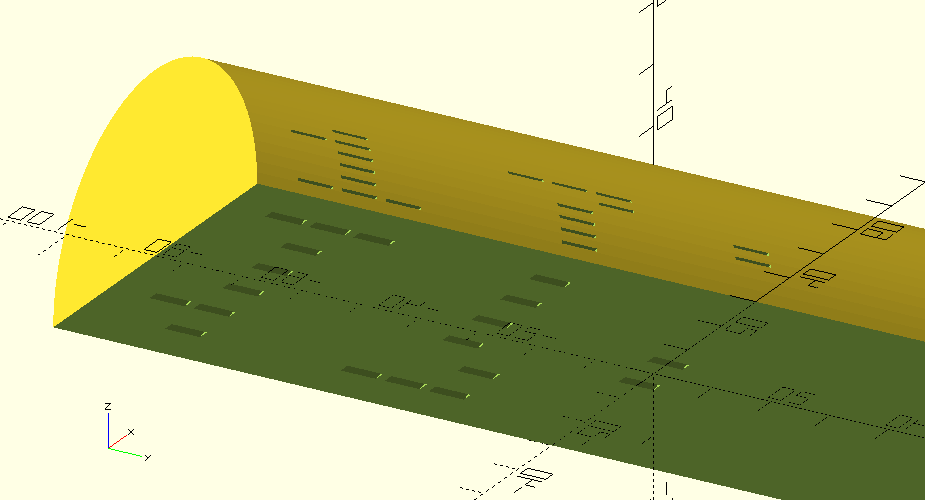
\includegraphics[width=.8\textwidth]{imagenes/17_00}
  \caption{Cecilia temía infundadamente que \lstinline!hora_solar! no
    superara la prueba de las 17:00.}
  \label{fig:17_00}
\end{figure}


Cecilia sintió, una vez más y ahora ante la figura \ref{fig:17_00},
que sus mejillas se encendían de rubor: ¿cómo fue capaz de desconfiar
de sus fórmulas y ecuaciones? ¡No podían fallar! Los rayos respondían
fielmente y con seguridad, sin importar el ángulo solicitado. Giró
para mirar a Antonia, a quien encontró con una sonrisa en la que
flotaba una tierna comprensión: seguramente ella también había pasado
(o quizá seguía sintiendo, alguna que otra vez) esas breves aunque
inquietantes desconfianzas.

\subsection{Los minutos}

---¡Es hora de ir a por los minutos! ---propuso Cecilia, agitando
ligeramente la cabeza como si quisiera despejarla de sus últimas
inquietudes---. Están ubicados simétricamente con respecto a las
horas; yo diría que la cosa ya está prácticamente resuelta:

\begin{lstlisting}
module hora_solar(horas,minutos){
  alfa=alfa(horas+minutos/60);
  hora_decenas=n_a_digito(horas,1);
  hora_unidades=n_a_digito(horas,0);
  minuto_decenas=n_a_digito(minutos,1);
  minuto_unidades=n_a_digito(minutos,0);                    
  delta_y=ancho_pixel+delta_ancho;
  // horas                    
  translate([0,-8.5*delta_y,0])
    digito(alfa,hora_decenas);
  translate([0,-3.5*delta_y,0])
    digito(alfa,hora_unidades);  
  // minutos
  translate([0,3.5*delta_y,0])
    digito(alfa,minuto_decenas);
  translate([0,8.5*delta_y,0])
    digito(alfa,minuto_unidades);  
}
difference(){
  cuerpo(170);
  separador(12,34);
  hora_solar(12,34);
}
\end{lstlisting}%

\begin{figure}[ht]
  \centering
  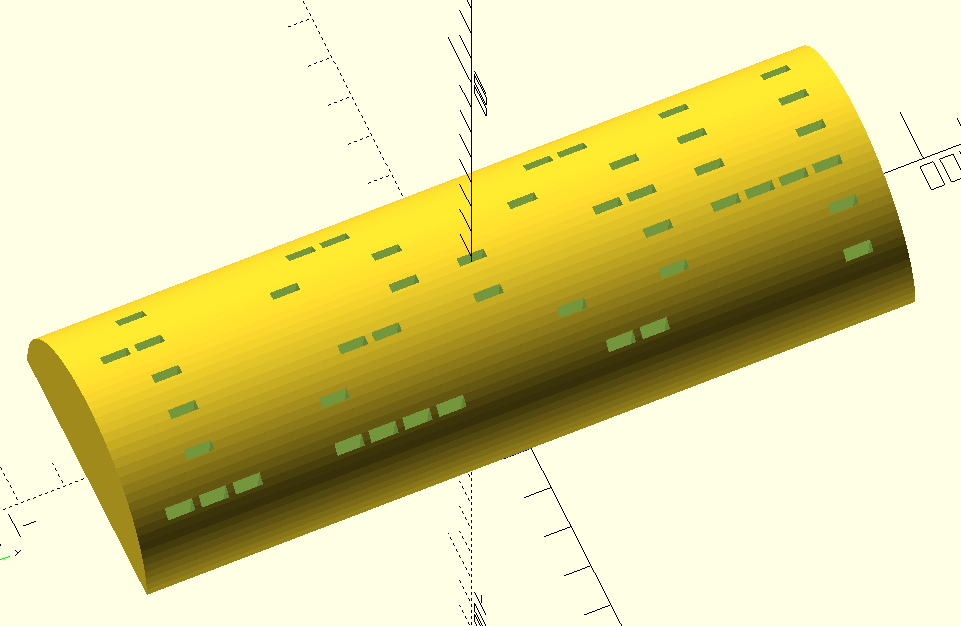
\includegraphics[width=.8\textwidth]{imagenes/12_34}
  \caption{Cecilia estampa las \texttt{12:34}.}
  \label{fig:12_34}
\end{figure}
  

Contemplando embelesada la figura \ref{fig:12_34}, Cecilia sintió que
la programación no podría hacerla nunca más dichosa que en ese
momento.

\subsection{Un cero inicial}

---¿No te parece un poco artificial la aparición de un cero en las
horas previas a las 10:00? ---preguntó Antonia, con una clara
entonación retórica, mientras recobraba el teclado.

\begin{lstlisting}
difference(){
  cuerpo(170);
  separador(8,53);
  hora_solar(8,53);
}
\end{lstlisting}%

\begin{figure}[ht]
  \centering
  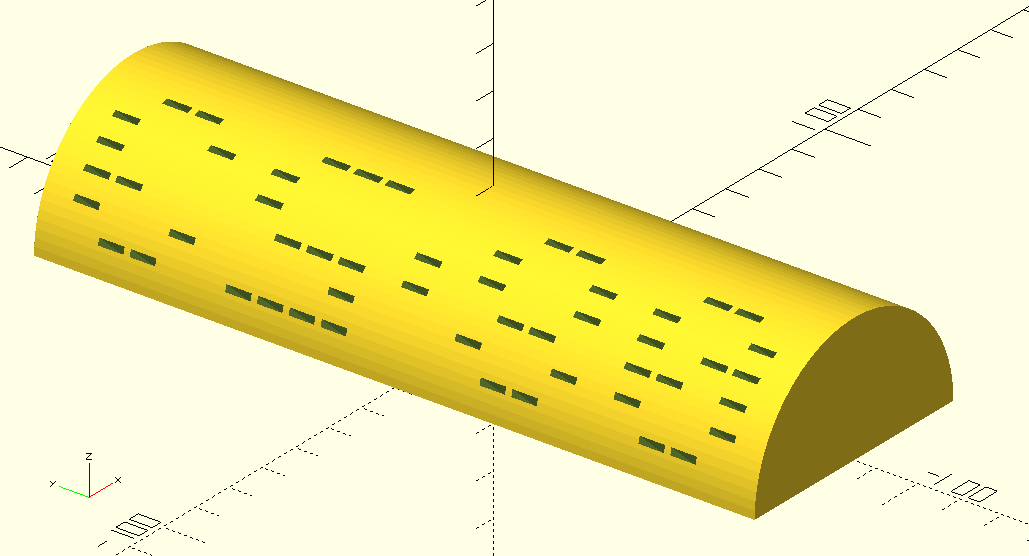
\includegraphics[width=.75\textwidth]{imagenes/08_53}
  \caption{Antonia opina que las 8:53 no deberían ostentar un cero
    inicial.}
  \label{fig:08_53}
\end{figure}
  

---¿Sugerís que suprimamos la aparición del mismo? ---pre\-gun\-tó a su
vez Cecilia, dando a entender que le parecía una buena idea, y tomando
el teclado.

\begin{lstlisting}
module hora_solar(horas,minutos){
  alfa=alfa(horas+minutos/60);
  hora_decenas=n_a_digito(horas,1);
  hora_unidades=n_a_digito(horas,0);
  minuto_decenas=n_a_digito(minutos,1);
  minuto_unidades=n_a_digito(minutos,0);                    
  delta_y=ancho_pixel+delta_ancho;
  // horas    
  if (hora_decenas != 0)
    translate([0,-8.5*delta_y,0])
      digito(alfa,hora_decenas);
  translate([0,-3.5*delta_y,0])
    digito(alfa,hora_unidades);  
  // minutos
  translate([0,3.5*delta_y,0])
    digito(alfa,minuto_decenas);
  translate([0,8.5*delta_y,0])
    digito(alfa,minuto_unidades);  
}
difference(){
  cuerpo(170);
  separador(8,53);
  hora_solar(8,53);
}
\end{lstlisting}%

\begin{figure}[ht]
  \centering
  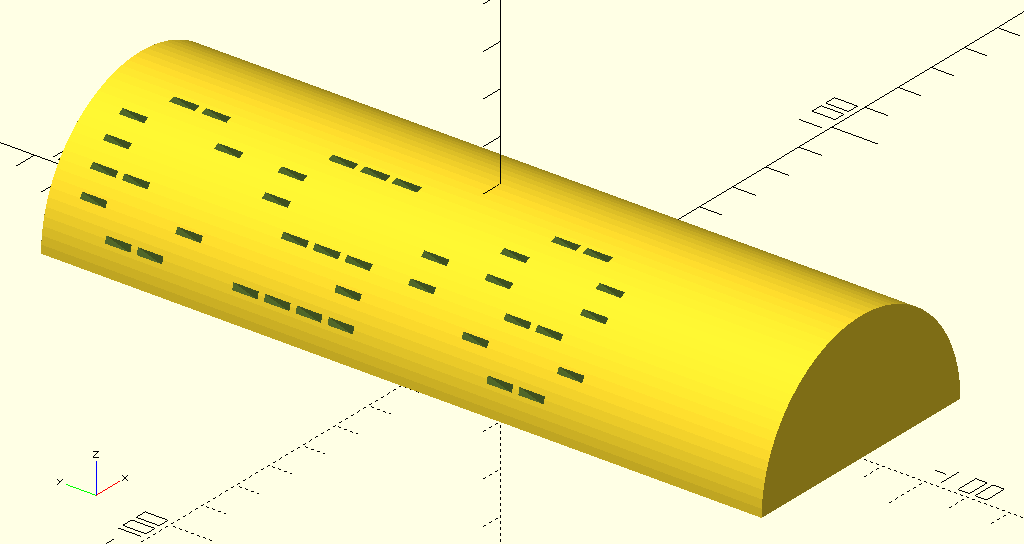
\includegraphics[width=.75\textwidth]{imagenes/8_53}
  \caption{Cecilia omite el `\texttt{0}' en las horas previas a las
    10:00.}
  \label{fig:8_53}
\end{figure}
  

Cecilia contempló su último retoque del texto con indisimulada
satisfacción: en la línea 9 indagaba si las decenas de la hora eran
distintas de cero; sólo en ese caso se horadaba el cuerpo del reloj
con el correspondiente dígito. Por las dudas lo probó con una hora
posterior a las 10:00:


\begin{lstlisting}
difference(){
  cuerpo(170);
  separador(14,39);
  hora_solar(14,39);
}
\end{lstlisting}

\begin{figure}[ht]
  \centering
  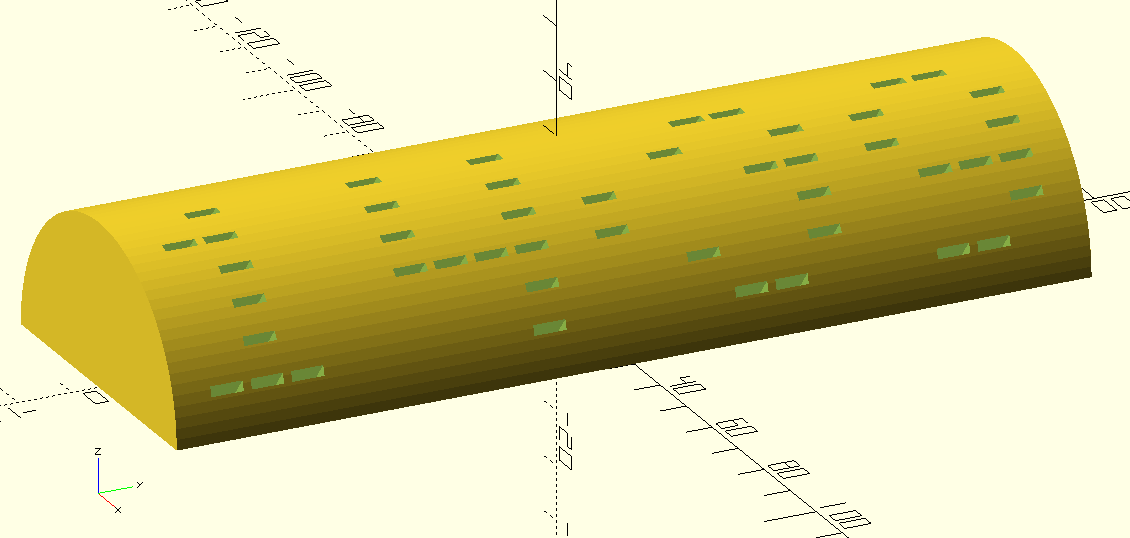
\includegraphics[width=.75\textwidth]{imagenes/14_39}
  \caption{Cecilia, prudentemente, confirma que las decenas de las
    horas se siguen mostrando para las horas posteriores a las 10:00.}
  \label{fig:14_39}
\end{figure}
  

Todo seguía en orden.

\section{El separador -- II}

Antonia y Cecilia contemplaban en silencio su obra; cualquiera que las
viese no hubiera podido distinguir si estaban serenamente felices por
el claro resultado conquistado o íntimamente inquietas en busca de
algún detalle para mejorar o agregar. Quizá se debatieran entre ambos
sentimientos.

---Creo que el \lstinline!separador! es parte de la
\lstinline!hora_solar!; debería pertenecer a este módulo ---soltó
Antonia suavemente.

Cecilia asintió en silencio, mientras se disponía a escribir:

\begin{lstlisting}
module hora_solar(horas,minutos){
  alfa=alfa(horas+minutos/60);
  hora_decenas=n_a_digito(horas,1);
  hora_unidades=n_a_digito(horas,0);
  minuto_decenas=n_a_digito(minutos,1);
  minuto_unidades=n_a_digito(minutos,0);                    
  delta_y=ancho_pixel+delta_ancho;
  // horas    
  if (hora_decenas != 0)
    translate([0,-8.5*delta_y,0])
      digito(alfa,hora_decenas);
  translate([0,-3.5*delta_y,0])
    digito(alfa,hora_unidades);  
  // minutos
  translate([0,3.5*delta_y,0])
    digito(alfa,minuto_decenas);
  translate([0,8.5*delta_y,0])
    digito(alfa,minuto_unidades);  
  // separador
  separador(horas,minutos);
}
difference(){
  cuerpo(170);
  hora_solar(13,46);
}
\end{lstlisting}%

  

Cecilia y Antonia se sentían cada vez más felices. Mientras tanto, un
nuevo \emph{bug} que las acechaba desde el capítulo
\ref{cap:el-primer-rayo-de-sol-i} las esperaba con impaciencia en el
próximo.

%\iftoggle{libro}{}{\clearpage} % comentar para ebook

\begin{figure}[ht]
  \centering
  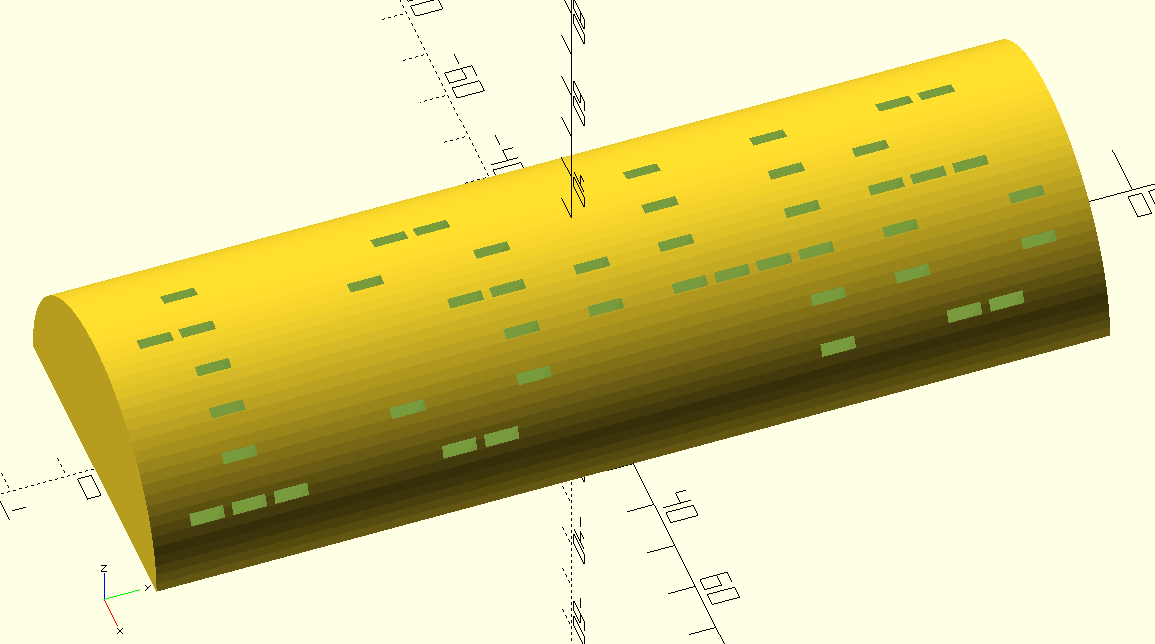
\includegraphics[width=.9\textwidth]{imagenes/13_46}
  \caption{Cecilia y Antonia comprueban una vez más el funcionamiento
    del módulo \lstinline!hora_solar!, ajenas por el momento a la
    inminente manifestación, en el capítulo siguiente, de un oscuro
    \emph{bug} escondido en su texto.}\iftoggle{libro}{\vspace{128in}}{}
  \label{fig:13_46}
\end{figure}

%%% Local Variables:
%%% mode: latex
%%% TeX-master: "../libro"
%%% End:
